\documentclass[11pt,table]{beamer}
\mode<presentation>
\usepackage{etex}
\usepackage{graphicx}
\usepackage{epstopdf}
\usepackage[english]{babel}
\usepackage{tabularx}
\usepackage{booktabs}
\usepackage{mathrsfs}
\usepackage{multicol}
\usepackage{bm}
\usepackage{subcaption}
\usepackage{wrapfig}
\usepackage{dcolumn}
\usepackage{threeparttable}
\usepackage{booktabs}
\usepackage{bbm}
\usepackage{amsmath,dsfont,listings}
\usepackage{amssymb}
\usepackage{rotating}
\usepackage{multirow}
\usepackage{tcolorbox}
\usepackage[authoryear]{natbib}
\usepackage{circledsteps}
\usepackage{qtree}

\usepackage{tikz}
\usetikzlibrary{arrows,decorations.pathmorphing,backgrounds,fit,positioning,shapes.symbols,chains}
\setbeamertemplate{section in toc}[sections numbered]
\setbeamertemplate{caption}[numbered]

\bibliographystyle{Econometrica}

\setbeamersize{text margin right=3.5mm, text margin left=7.5mm}  % text margin
\setbeamersize{sidebar width left=0cm, sidebar width right=0mm}
\setbeamertemplate{sidebar right}{}
\setbeamertemplate{sidebar left}{}

\definecolor{text-grey}{rgb}{0.45, 0.45, 0.45} % grey text on white background
\definecolor{bg-grey}{rgb}{0.66, 0.65, 0.60} % grey background (for white text)
\definecolor{fu-blue}{RGB}{0, 51, 102} % blue text
\definecolor{fu-green}{RGB}{153, 204, 0} % green text
\definecolor{fu-red}{RGB}{204, 0, 0} % red text (used by \alert)
\definecolor{BrewerBlue}{HTML}{377EB8} % Define Brewer Blue
\definecolor{BrewerRed}{HTML}{E41A1C}  % Define Brewer Red

\setbeamertemplate{frametitle}{%
    \vskip-30pt \color{text-grey}\large%
    \begin{minipage}[b][23pt]{\textwidth}%
    \flushleft\insertframetitle%
    \end{minipage}%
}

\setbeamertemplate{navigation symbols}{} 

%%% begin title page
\setbeamertemplate{title page}{
\vskip2pt\hfill
\vskip19pt\hskip3pt

% set the title and the author
\vskip4pt
\parbox[top][1.35cm][c]{11cm}{\LARGE\color{text-grey} \textcolor{red1}{RL}earning:\\[1ex] \inserttitle \\[1ex] \small \quad \\[3ex]}
\vskip17pt
\parbox[top][1.35cm][c]{11cm}{\small Unit 4-5: \insertsubtitle \\[2ex] \insertauthor \\[1ex]}
}
%%% end title page

%%% colors
\usecolortheme{lily}
\setbeamercolor*{normal text}{fg=black,bg=white}
\setbeamercolor*{alerted text}{fg=fu-red}
\setbeamercolor*{example text}{fg=fu-green}
\setbeamercolor*{structure}{fg=fu-blue}

\setbeamercolor*{block title}{fg=white,bg=black!50}
\setbeamercolor*{block title alerted}{fg=white,bg=black!50}
\setbeamercolor*{block title example}{fg=white,bg=black!50}

\setbeamercolor*{block body}{bg=black!10}
\setbeamercolor*{block body alerted}{bg=black!10}
\setbeamercolor*{block body example}{bg=black!10}

\setbeamercolor{bibliography entry author}{fg=fu-blue}
\setbeamercolor{bibliography entry journal}{fg=text-grey}
\setbeamercolor{item}{fg=fu-blue}
\setbeamercolor{navigation symbols}{fg=text-grey,bg=bg-grey}
%%% end colors

%%% headline
\setbeamertemplate{headline}{
\vskip30pt
}
%%% end headline

%%% footline
\newcommand{\footlinetext}{
%\insertshortinstitute, \insertshorttitle, \insertshortdate
}
\setbeamertemplate{footline}{
\vskip2pt
\hfill \raisebox{-1pt}{\usebeamertemplate***{navigation symbols}}
\hfill \insertframenumber\hspace{10pt}
\vskip4pt
}
%%% end footline

%%% settings for listings package
\lstset{extendedchars=true, showstringspaces=false, basicstyle=\footnotesize\sffamily, tabsize=2, breaklines=true, breakindent=10pt, frame=l, columns=fullflexible}
\lstset{language=Java} % this sets the syntax highlighting
\lstset{mathescape=true} % this switches on $...$ substitution in code
% enables UTF-8 in source code:
\lstset{literate={ä}{{\"a}}1 {ö}{{\"o}}1 {ü}{{\"u}}1 {Ä}{{\"A}}1 {Ö}{{\"O}}1 {Ü}{{\"U}}1 {ß}{\ss}1}
%%% end listings

\usepackage{concmath}
\usepackage{xcolor}
\definecolor{red1}{RGB}{206, 17, 38}
\definecolor{blue1}{RGB}{16, 118, 208}
\definecolor{gray1}{RGB}{117, 115, 115}
\usepackage{hyperref}


\newtheorem{proposition}{Proposition}
\newtheorem{assumption}{Definition}

\title[]{Short guides to reinforcement learning}
\subtitle[]{Actor Critic Algorithms}
\author[D. Rostam-Afschar]{\textcolor{gray1}{Davud Rostam-Afschar (Uni Mannheim)}}
\date[]{\today}
\subject{Econometrics}
\renewcommand{\footlinetext}{\insertshortinstitute, \insertshorttitle, \insertshortdate}
\hypersetup{
    bookmarks=false,
    unicode=false,
    pdftoolbar=false,
    pdffitwindow=true,
    pdftitle={Reinforcement Learning for Business, Economics, and Social Sciences: \insertsubtitle},
    pdfauthor={Davud Rostam-Afschar},
    pdfsubject={Reinforcement Learning},
    pdfkeywords={reinforcement learning, Actor Critic Algorithms},
    pdfnewwindow=true,
}
\def\sym#1{\ifmmode^{#1}\else\(^{#1}\)\fi}

\begin{document}

\begin{frame}[plain]
  \titlepage
\end{frame}

% --------------------------------------------------- Slide --
%\begin{frame}
	%\frametitle{Content}
	%\tableofcontents[]
%\end{frame}

\section{Introduction to Reinforcement Learning}
{
\setbeamercolor{background canvas}{bg=BrewerBlue}
\begin{frame}
\centering
\Huge
\textcolor{white}{Learn acting via policy gradient---\\evaluate actions via TD\\... or the advantage}
\thispagestyle{empty}
\end{frame}
}




\begin{frame}
\frametitle{Actor Critic}

\begin{itemize}
    \item Q-learning
    \begin{itemize}
        \item Model-free value-based method
        \item No explicit policy representation\\[2ex]
    \end{itemize}
    
    \item Policy gradient
    \begin{itemize}
        \item Model-free policy-based method
        \item No explicit value function representation\\[2ex]
    \end{itemize}
    
    \item \textbf{Actor Critic}
    \begin{itemize}
        \item \textcolor{red1}{Model-free policy and value based method}
    \end{itemize}
\end{itemize}

\end{frame}


\section{Stochastic Gradient Policy with a Baseline}
{
\setbeamercolor{background canvas}{bg=BrewerBlue}
\begin{frame}
\centering
\Huge
\textcolor{white}{Stochastic Gradient Policy\\... with a Baseline}
\thispagestyle{empty}
\end{frame}
}


\begin{frame}
\frametitle{Stochastic Gradient Policy Theorem}

\begin{itemize}
    \item Stochastic Gradient Policy Theorem
\end{itemize}

\[
\nabla V_\theta(s_0) \propto \sum_s \mu_\theta(s) \sum_a \nabla \pi_\theta(a|s) Q_\theta(s,a)
\]

\begin{itemize}
    \item Equivalent Stochastic Gradient Policy Theorem with a baseline \( b(s) \)
\end{itemize}

\[
\nabla V_\theta(s_0) \propto \sum_s \mu_\theta(s) \sum_a \nabla \pi_\theta(a|s) \left[ Q_\theta(s,a) - \textcolor{red1}{b(s)} \right]
\]
\footnotesize
\[
\text{since} \quad \sum_a \nabla \pi_\theta(a|s) \textcolor{red1}{b(s)} = b(s) \nabla \sum_a \pi_\theta(a|s) = b(s) \nabla 1 = 0
\]

\end{frame}



\begin{frame}
\frametitle{Baseline}

\begin{itemize}
    \item Baseline often chosen to be \( b(s) \approx V^\pi(s) \)
    \item Advantage function: \( A(s,a) = Q(s,a) - V^\pi(s) \)
    \item Gradient update:
\end{itemize}

\[
\theta \leftarrow \theta + \alpha \gamma^n A(s_n, a_n) \nabla \log \pi_\theta(a_n|s_n)
\]

\begin{itemize}
    \item Benefit: faster empirical convergence
\end{itemize}

\end{frame}



\section{REINFORCE Algorithm with a baseline}
{
\setbeamercolor{background canvas}{bg=BrewerBlue}
\begin{frame}
\centering
\Huge
\textcolor{white}{REINFORCE Algorithm\\ with a baseline}
\thispagestyle{empty}
\end{frame}
}

\begin{frame}
\frametitle{REINFORCE Algorithm with a baseline}

\begin{tcolorbox}[colframe=black, boxrule=1pt, sharp corners]

\textcolor{red1}{REINFORCEwithBaseline(\( s_0, \pi_\theta \))}

Initialize \( \pi_\theta \) to anything\\
Initialize \( V_w \) to anything\\
Loop forever (for each episode)
\begin{itemize}
    \item[] Generate episode \( s_0, a_0, r_0, s_1, a_1, r_1, \dots, s_T, a_T, r_T \) with \( \pi_\theta \)
    \item[] Loop for each step of the episode \( n = 0, 1, \dots, T \)
    \begin{itemize}
        \item[] \( G_n \leftarrow \sum_{t=0}^{T-n} \gamma^{t} r_{n+t} \)
        \item[] \textcolor{red1}{\( \delta \leftarrow G_n - V_w(s_n) \)}
        \item[] Update value function: \( w \leftarrow w + \alpha_w \gamma^n \textcolor{red1}{\delta} \nabla V_w(s_n) \)
        \item[] Update policy: \( \theta \leftarrow \theta + \alpha_\theta \gamma^n \textcolor{red1}{\delta} \nabla \log \pi_\theta(a_n|s_n) \)
    \end{itemize}
\end{itemize}

Return \( \pi_\theta \)

\end{tcolorbox}

\end{frame}


\begin{frame}
\frametitle{Performance Comparison}

\begin{figure}
	\centering
		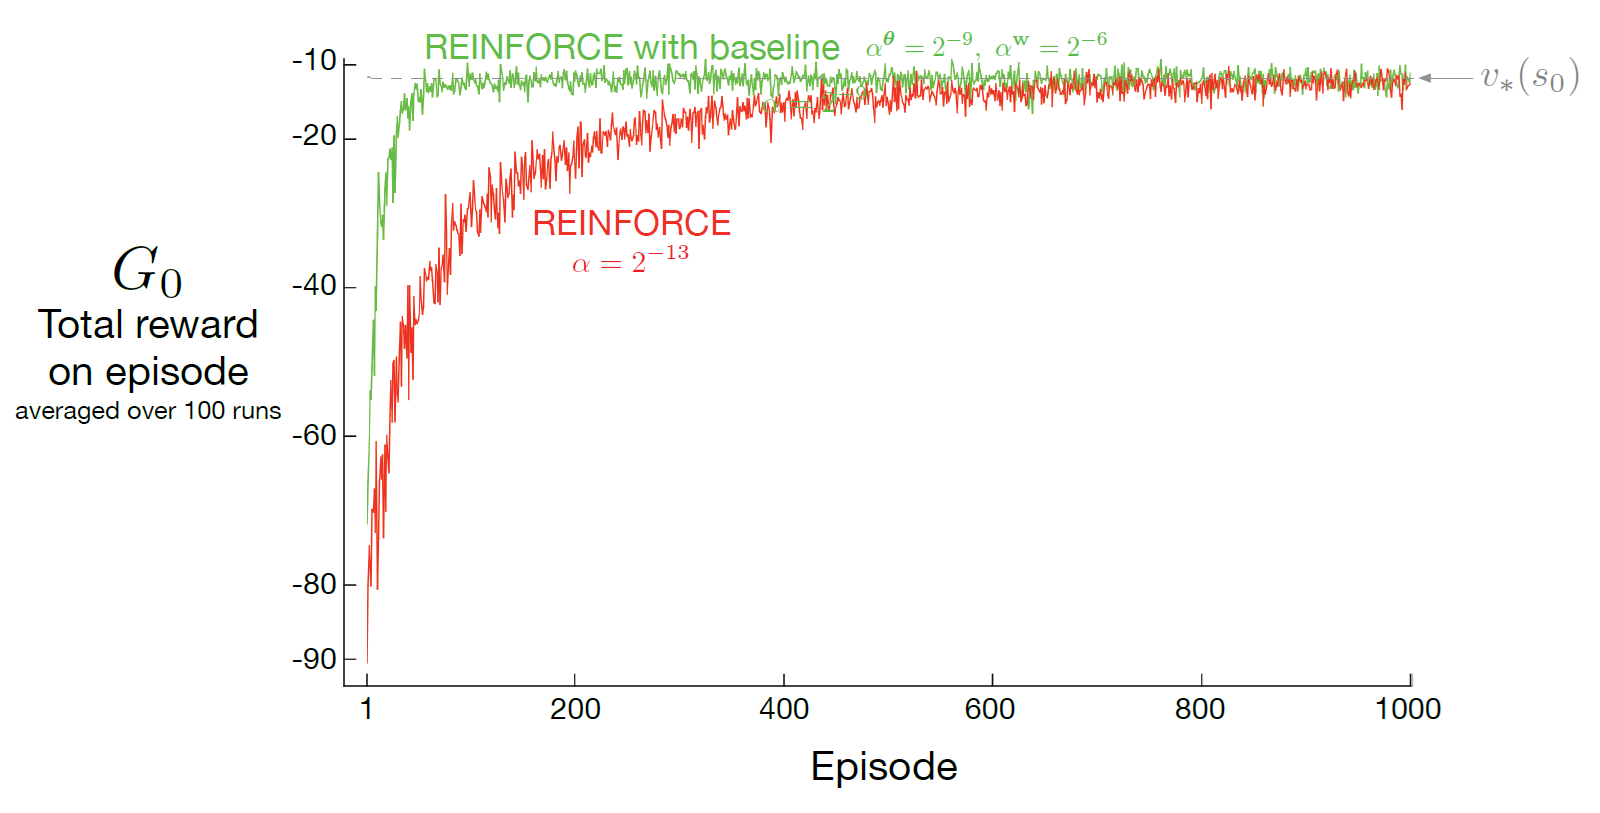
\includegraphics[width=1.00\textwidth]{figures/1}
	\label{fig:1}
\end{figure}


\end{frame}

\begin{frame}
\frametitle{Temporal difference update}

\begin{itemize}
    \item Instead of updating \( V(s) \) by Monte Carlo sampling
\end{itemize}

\[
\delta \leftarrow G_n - V_w(s_n)
\]

\begin{itemize}
    \item Bootstrap with temporal difference updates
\end{itemize}

\[
\delta \leftarrow r_n + \gamma V_w(s_{n+1}) - V_w(s_n)
\]

\begin{itemize}
    \item Benefit: reduced variance (faster convergence)
\end{itemize}

\end{frame}



\begin{frame}
\frametitle{Actor Critic Algorithm}

\begin{tcolorbox}[colframe=black, boxrule=1pt, sharp corners]

\textcolor{red1}{ActorCritic(\( s_0, \pi_\theta \))}


Initialize \( \pi_\theta \) to anything\\
Initialize \( Q_w \) to anything\\
Loop forever (for each episode)
\begin{itemize}
    \item[] Initialize \( s_0 \) and set \( n \leftarrow 0 \)
    \item[] Loop while \( s \) is not terminal (for each time step \( n \))
    \begin{itemize}
        \item[] Sample \( a_n \sim \pi_\theta(a|s_n) \)
        \item[] Execute \( a_n \), observe \( s_{n+1} \), \( r_n \)
        \item[] \textcolor{red1}{\( \delta \leftarrow r_n + \gamma V_w(s_{n+1}) - V_w(s_n) \)}
        \item[] Update \textcolor{red1}{value} function: \( w \leftarrow w + \alpha_w \gamma^n \textcolor{red1}{\delta} \nabla V_w(s_n) \)
        \item[] Update \textcolor{red1}{policy}: \( \theta \leftarrow \theta + \alpha_\theta \gamma^n \textcolor{red1}{\delta} \nabla \log \pi_\theta(a_n|s_n) \)
        \item[] \( n \leftarrow n + 1 \)
    \end{itemize}
\end{itemize}

Return \( \pi_\theta \)

\end{tcolorbox}

\end{frame}

\begin{frame}
\frametitle{Advantage update}

\begin{itemize}
    \item Instead of doing temporal difference updates
\end{itemize}

\[
\delta \leftarrow r_n + \gamma V_w(s_{n+1}) - V_w(s_n)
\]

\vspace{0.5em}

\begin{itemize}
    \item Update with the advantage function
\end{itemize}

\[
A(s_n, a_n) \leftarrow r_n + \gamma \max_{a_{n+1}} Q(s_{n+1}, a_{n+1}) - \textcolor{red1}{\sum_a \pi_\theta(a|s_n) Q(s_n, a)}
\]

\[
\theta \leftarrow \theta + \alpha_\theta \gamma^n A(s_n, a_n) \nabla \log \pi_\theta(a_n|s_n)
\]

\vspace{0.5em}

\begin{itemize}
    \item Benefit: faster convergence
\end{itemize}

\end{frame}


\section{Advantage Actor Critic (A2C)}
{
\setbeamercolor{background canvas}{bg=BrewerBlue}
\begin{frame}
\centering
\Huge
\textcolor{white}{Advantage Actor Critic (A2C)}
\thispagestyle{empty}
\end{frame}
}

\begin{frame}
\frametitle{Advantage Actor Critic (A2C)}

\begin{tcolorbox}[colframe=black, boxrule=1pt, sharp corners]

\textcolor{red1}{A2C($s, \pi_\theta$)}

Initialize \( \pi_\theta \) to anything\\
Loop forever (for each episode)\\
Initialize \( s_0 \) and set \( n \leftarrow 0 \)
\begin{itemize}
    \item[] Loop while \( s \) is not terminal (for each time step \( n \))
    \begin{itemize}
        \item[] Select \( a_n \)
        \item[] Execute \( a_n \), observe \( s_{n+1}, r_n \)
        \item[] \( \delta \leftarrow r_n + \gamma \max_{a'} Q_w(s_{n+1}, a') - Q_w(s_n, a_n) \)
        \item[] \textcolor{red1}{\( A(s_n, a_n) \leftarrow r_n + \gamma \max_{a'} Q_w(s_{n+1}, a') - \sum_a \pi_\theta(a|s_n) Q_w(s_n, a) \)}
        \item[] Update \( Q \): \( w \leftarrow w + \alpha_w \gamma^n \delta \nabla_w Q_w(s_n, a_n) \)
        \item[] Update \( \pi \): \( \theta \leftarrow \theta + \alpha_\theta \gamma^n \textcolor{red1}{A(s_n, a_n)} \nabla \log \pi_\theta(a_n|s_n) \)
        \item[] \( n \leftarrow n + 1 \)
    \end{itemize}
\end{itemize}

\end{tcolorbox}

\end{frame}


\section{Deterministic Gradient Policy}
{
\setbeamercolor{background canvas}{bg=BrewerBlue}
\begin{frame}
\centering
\Huge
\textcolor{white}{Deterministic Gradient Policy}
\thispagestyle{empty}
\end{frame}
}


\begin{frame}
\frametitle{Continuous Actions}

\begin{itemize}
    \item Consider a deterministic policy \( \pi_\theta: s \rightarrow a \)
\end{itemize}

\vspace{0.5em}

\begin{itemize}
    \item Deterministic Gradient Policy Theorem
\end{itemize}

\[
\nabla V_\theta(s_0) \propto \mathbb{E}_{s \sim \mu_\theta} \left[ \nabla_\theta \pi_\theta(s) \nabla_a Q_\theta(s, a) \big|_{a=\pi_\theta(s)} \right]
\]

\begin{itemize}
    \item Proof: see Silver et al. 2014
\end{itemize}

\vspace{0.5em}

\begin{itemize}
    \item Stochastic Gradient Policy Theorem
\end{itemize}

\[
\nabla V_\theta(s_0) \propto \sum_s \mu_\theta(s) \sum_a \nabla_\theta \pi_\theta(a|s) Q_\theta(s,a)
\]

\end{frame}



\section{Deterministic Policy Gradient (DPG)}
{
\setbeamercolor{background canvas}{bg=BrewerBlue}
\begin{frame}
\centering
\Huge
\textcolor{white}{Deterministic Policy Gradient (DPG)}
\thispagestyle{empty}
\end{frame}
}

\begin{frame}
\frametitle{Deterministic Policy Gradient (DPG)}

\begin{tcolorbox}[colframe=black, boxrule=1pt, sharp corners]

\textcolor{red1}{DPG(\( s_0, \pi_\theta \))}

Initialize \( \pi_\theta \) to anything\\
Loop forever (for each episode)\\
Initialize \( s_0 \) and set \( n \leftarrow 0 \)
\begin{itemize}
    \item[] Loop while \( s \) is not terminal (for each time step \( n \))
    \begin{itemize}
        \item[] Select \( a_n = \pi_\theta(s_n) \)
        \item[] Execute \( a_n \), observe \( s_{n+1}, r_n \)
        \item[] \( \delta \leftarrow r_n + \gamma Q_w\left( s_{n+1}, \pi_\theta(s_{n+1}) \right) - Q_w(s_n, a_n) \)
        \item[] Update \( Q \): \( w \leftarrow w + \alpha_w \gamma^n \delta \nabla_w Q_w(s_n, a_n) \)
        \item[] Update \( \pi \): \( \theta \leftarrow \theta + \alpha_\theta \gamma^n \nabla_\theta \pi_\theta(s_n) \nabla_a Q_w(s_n, a_n) \big|_{a=\pi_\theta(s_n)} \)
        \item[] \( n \leftarrow n + 1 \)
    \end{itemize}
\end{itemize}

Return \( \pi_\theta \)

\end{tcolorbox}

\end{frame}




\begin{frame}[t,allowframebreaks
]\nocite{*}
\frametitle{References}
\small
\bibliography{bib}
\end{frame}
\section{Takeaways}
{
\setbeamercolor{background canvas}{bg=BrewerBlue}
\begin{frame}
\centering
\Huge
\textcolor{white}{Takeaways}
\thispagestyle{empty}
\end{frame}
}

\begin{frame}



\frametitle{Actor Critic algorithms}

\begin{itemize}
    \item Policy gradient methods can be improved with a baseline (value function)
    \item Actor Critic algorithms use a learned value function as the baseline
    \item Temporal difference updates reduce variance (faster convergence)
    \item Deterministic policy gradients can be used for continuous actions
\end{itemize}

\end{frame}



\end{document}
